\section{Overflow mode: RUN281}
%%%%%%%%%%%%%%%%%%%%%%%%%%%%%%%%%%%%%%%%%%%%%%%%%%%%%%%%%%%%%%%%%%%%%%%%%%%%%%
\subsection{Time distribution}
The analysis started examining the data time distribution of each channel.
After a preliminary observation of the distributions, we saw different patterns for channels in the first FPGA and in the second FPGA,
as illustrated in Fig. \ref{fig:1}: the initial though  was the occurrence of a cessation in data acquisition for specific channels at a certain time.

\begin{figure}[H]
  \hspace{-0.5in}
  \begin{tikzpicture}
    \node[anchor=south west,inner sep=0] at (0,0.) {
      % \node[shift={(0 cm,0.cm)},inner sep=0,rotate={90}] at (0,0) {}
      % \makebox[\textwidth][c] {
      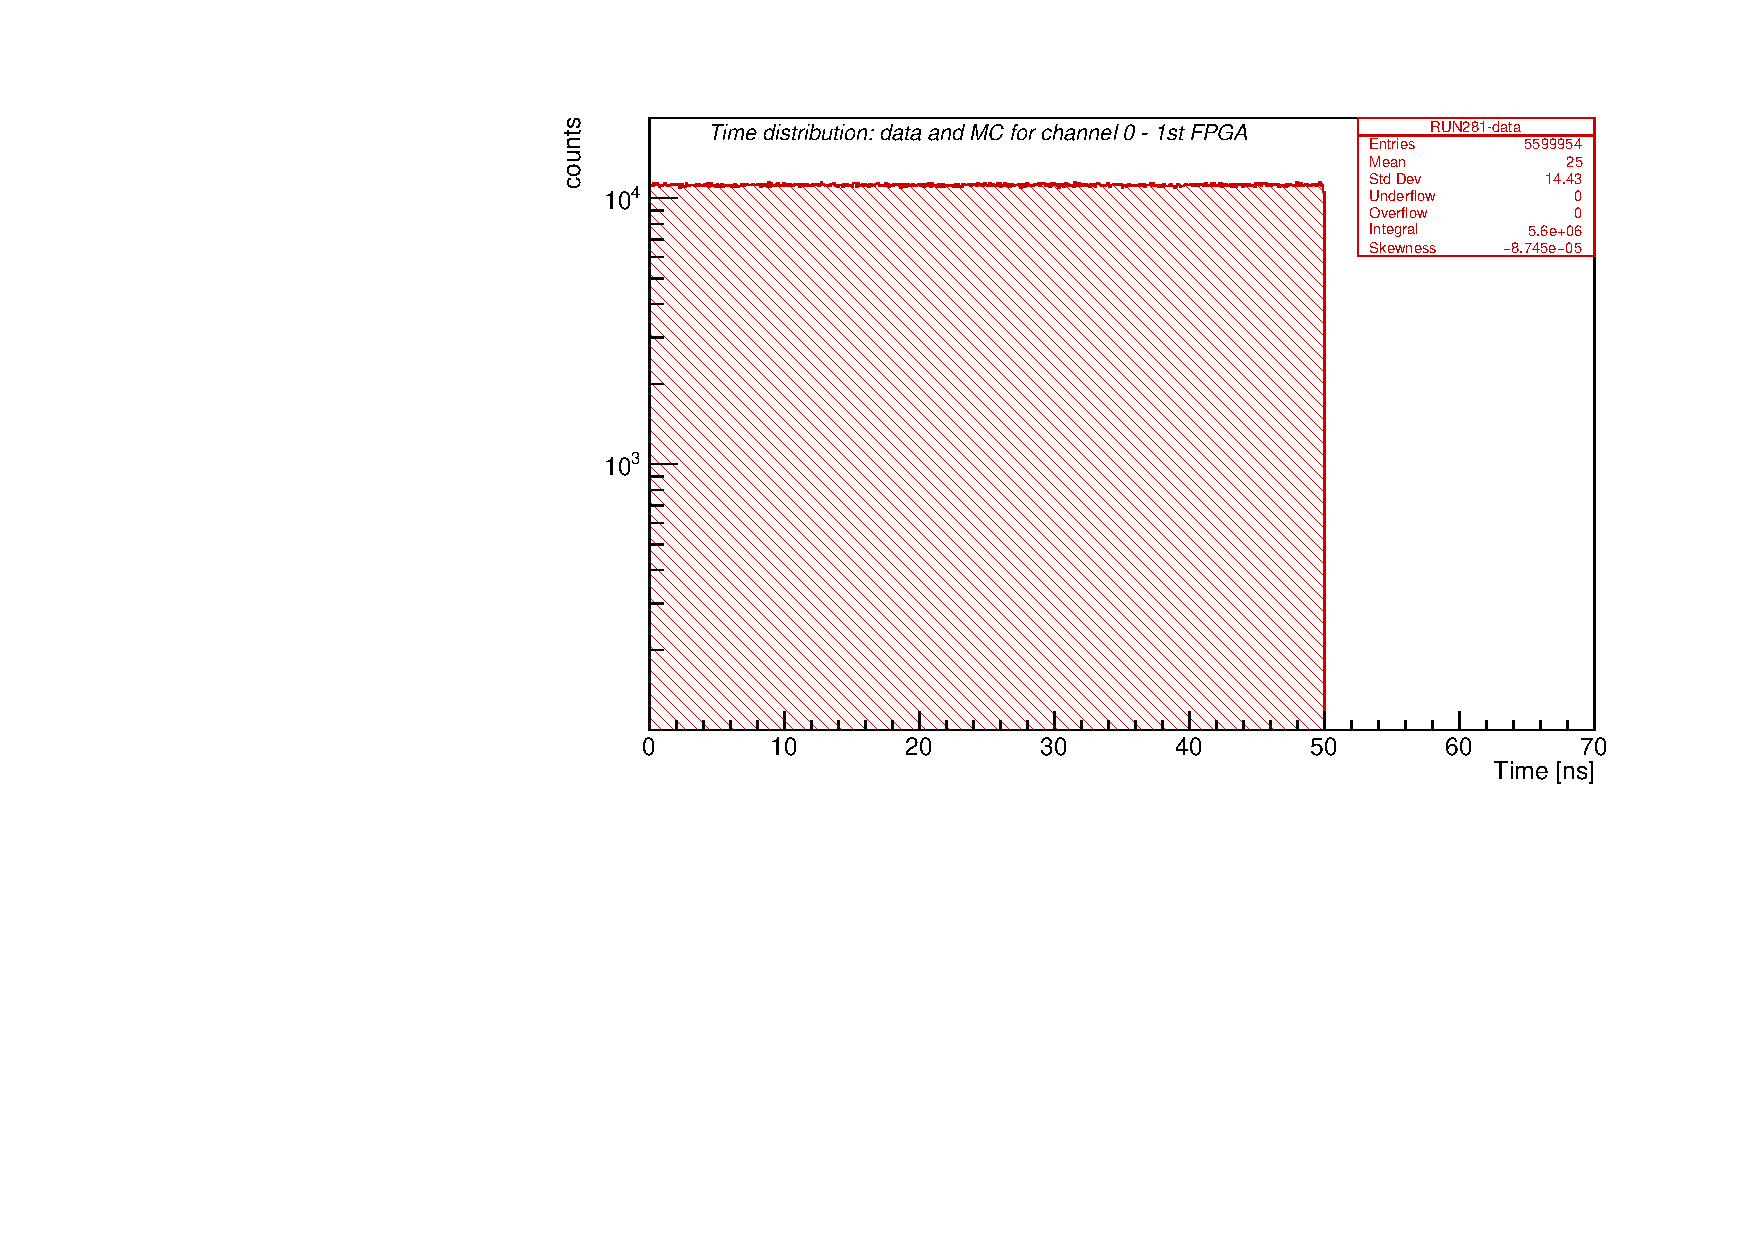
\includegraphics[width=0.5\textwidth]{figures/pdf/figure_00007_timedistr_roc_simulation_ch0_281}
      % }
    };
    \node[anchor=south west,inner sep=0] at (10,0.) {
      % \node[shift={(0 cm,0.cm)},inner sep=0,rotate={90}] at (0,0) {}
      % \makebox[\textwidth][c] {
      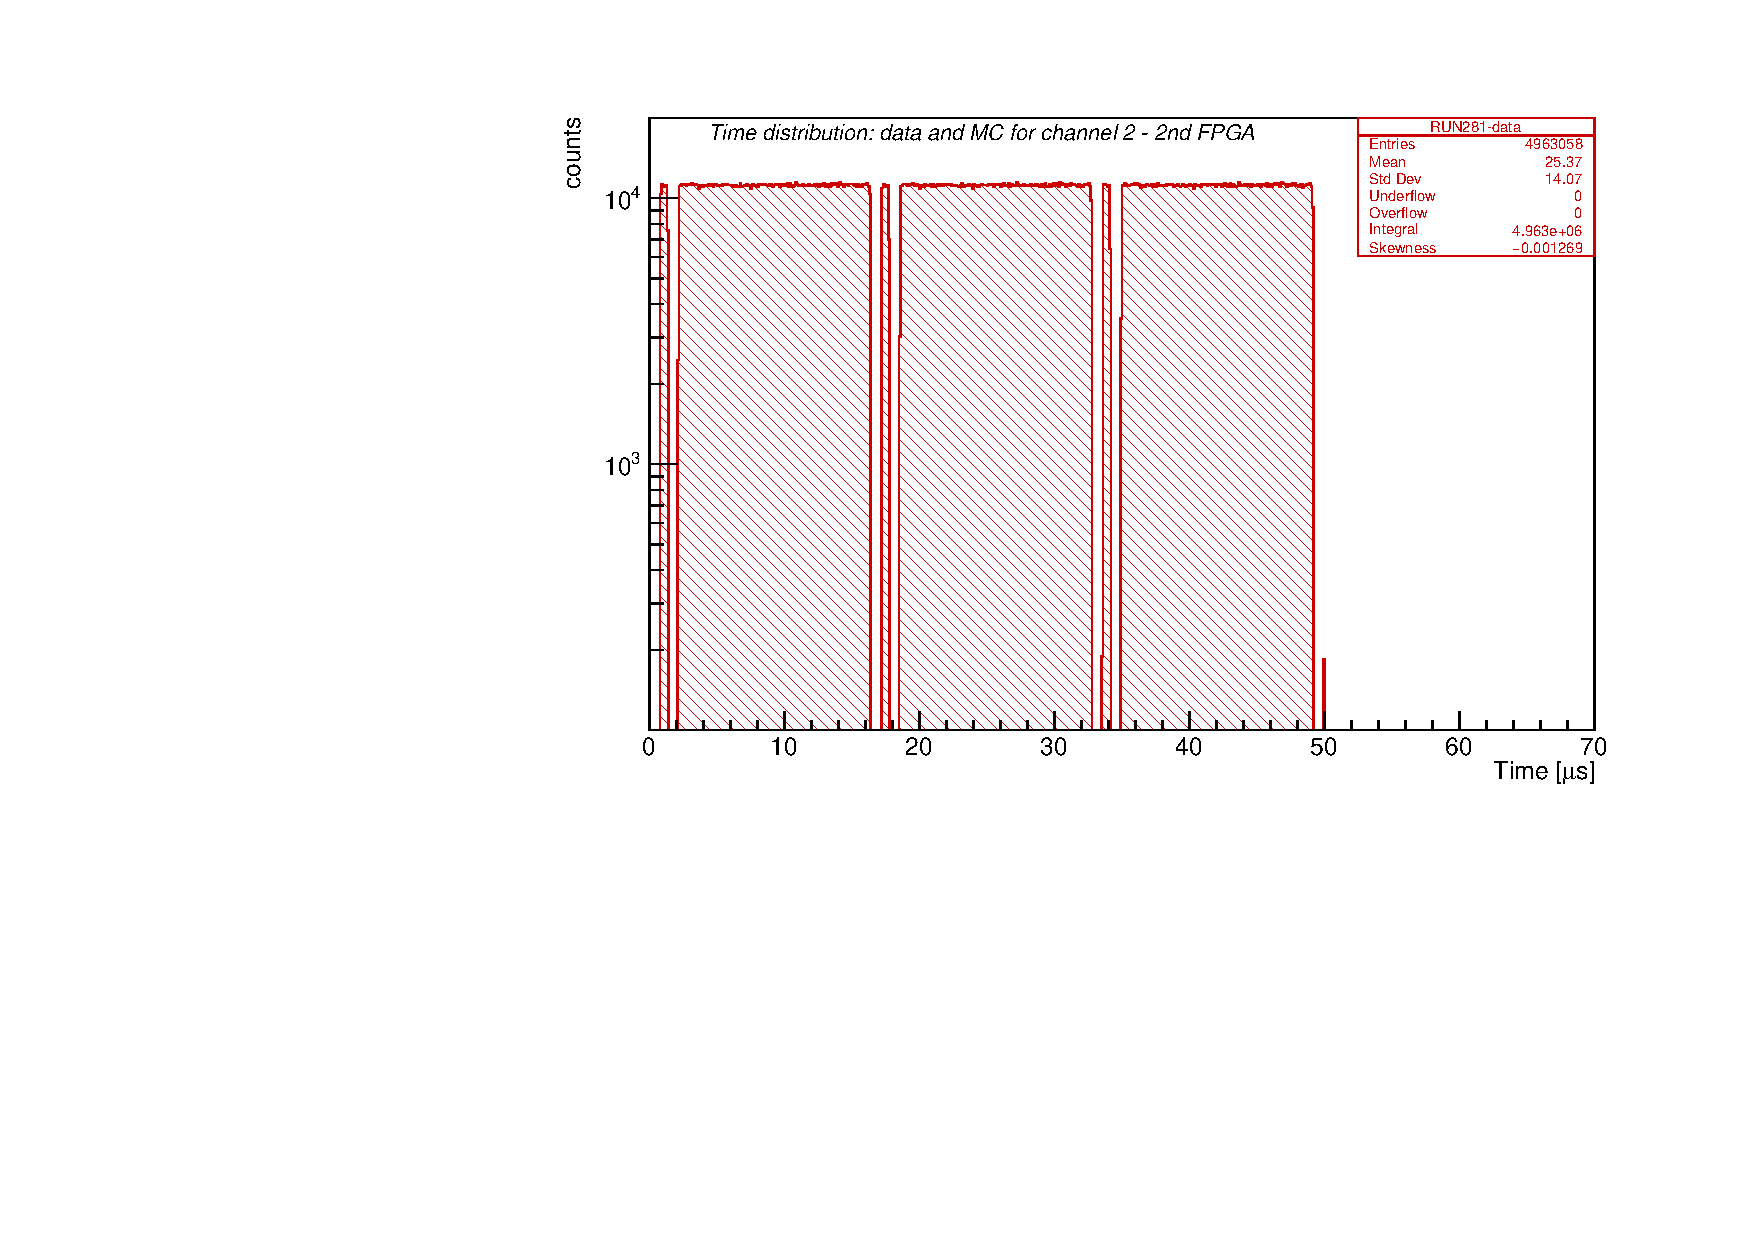
\includegraphics[width=0.5\textwidth]{figures/pdf/figure_00003_timedistr_roc_simulation_ch2_281}
      % }
    };
  \end{tikzpicture}
  \caption{
    \label{fig:1}
    right: First FPGA's channel time distribution, left: Second FPGA's channel time distribution.
  }
\end{figure}
We thought it was necessary to characterize the apparatus with a Monte Carlo simulation for our Data Acquisition (DAQ) system, in order to understand the interruptions,
so we redirect to section \ref{MonteCarlo} for further information.
\subsection{Occupancy: Number of hits versus channel}
We conducted an analysis by plotting the number of hits in each channel as a function of the channel number, which revealed a non-uniform distribution. 
Specifically, channels were arranged in an ascending order, spanning from channel 0 to channel 95.
As second step, we managed to generate a histogram with an alternative channel order, as we would expect the filling to occur.
Our expectation was to observe a declining trend in the number of hits per channel, primarily due to the progressive filling of the buffer. 
However, contrary to our initial hypothesis, we encountered a distinctive pattern in which the number of hits exhibited a decrease until reaching zero hits at a specific channel,
followed by a subsequent increase beyond the 72nd channel, which corresponds to channel 95.

Upon careful examination, we deduced that the initial channel ordering was incorrect. 
The first and the second lanes of the second FPGA were inverted and also some channels of the second FPGA.
Consequently, we have identified a revised channel sequence, verified also by the Monte Carlo simulation, which is as follows:
\begin{center}
\begin{tabular}{cc}
\textbf{FIST FPGA}: & \\
&91,85,79,73,67,61,55,49,\\
\textit{lane 1}: &43,37,31,25,19,13,7,1,\\
&90,84,78,72,66,60,54,48,\\
& \\
&42,36,30,24,18,12,6,0,\\
\textit{lane 2}: &93,87,81,75,69,63,57,51,\\
&45,39,33,27,21,15,9,3,\\
\textbf{SECOND FPGA}:&\\
&\\
&38,44,5,11,17,23,29,35,\\
\textit{lane 1}:&41,92,2,8,14,20,26,32,\\
&86,80,74,68,62,56,50,47,\\
 & \\
&95,89,83,22,16,28,34,40,\\
\textit{lane 2}:&46,53,59,65,71,77,10,4,\\
&94,88,82,76,70,64,58,52\\
\end{tabular}
\end{center}   
At this point we have plotted the number of hits versus the channel number in the order that the filling occurred, as we can see in Fig. \ref{fig:2}.
\begin{figure}[!h]
\centering
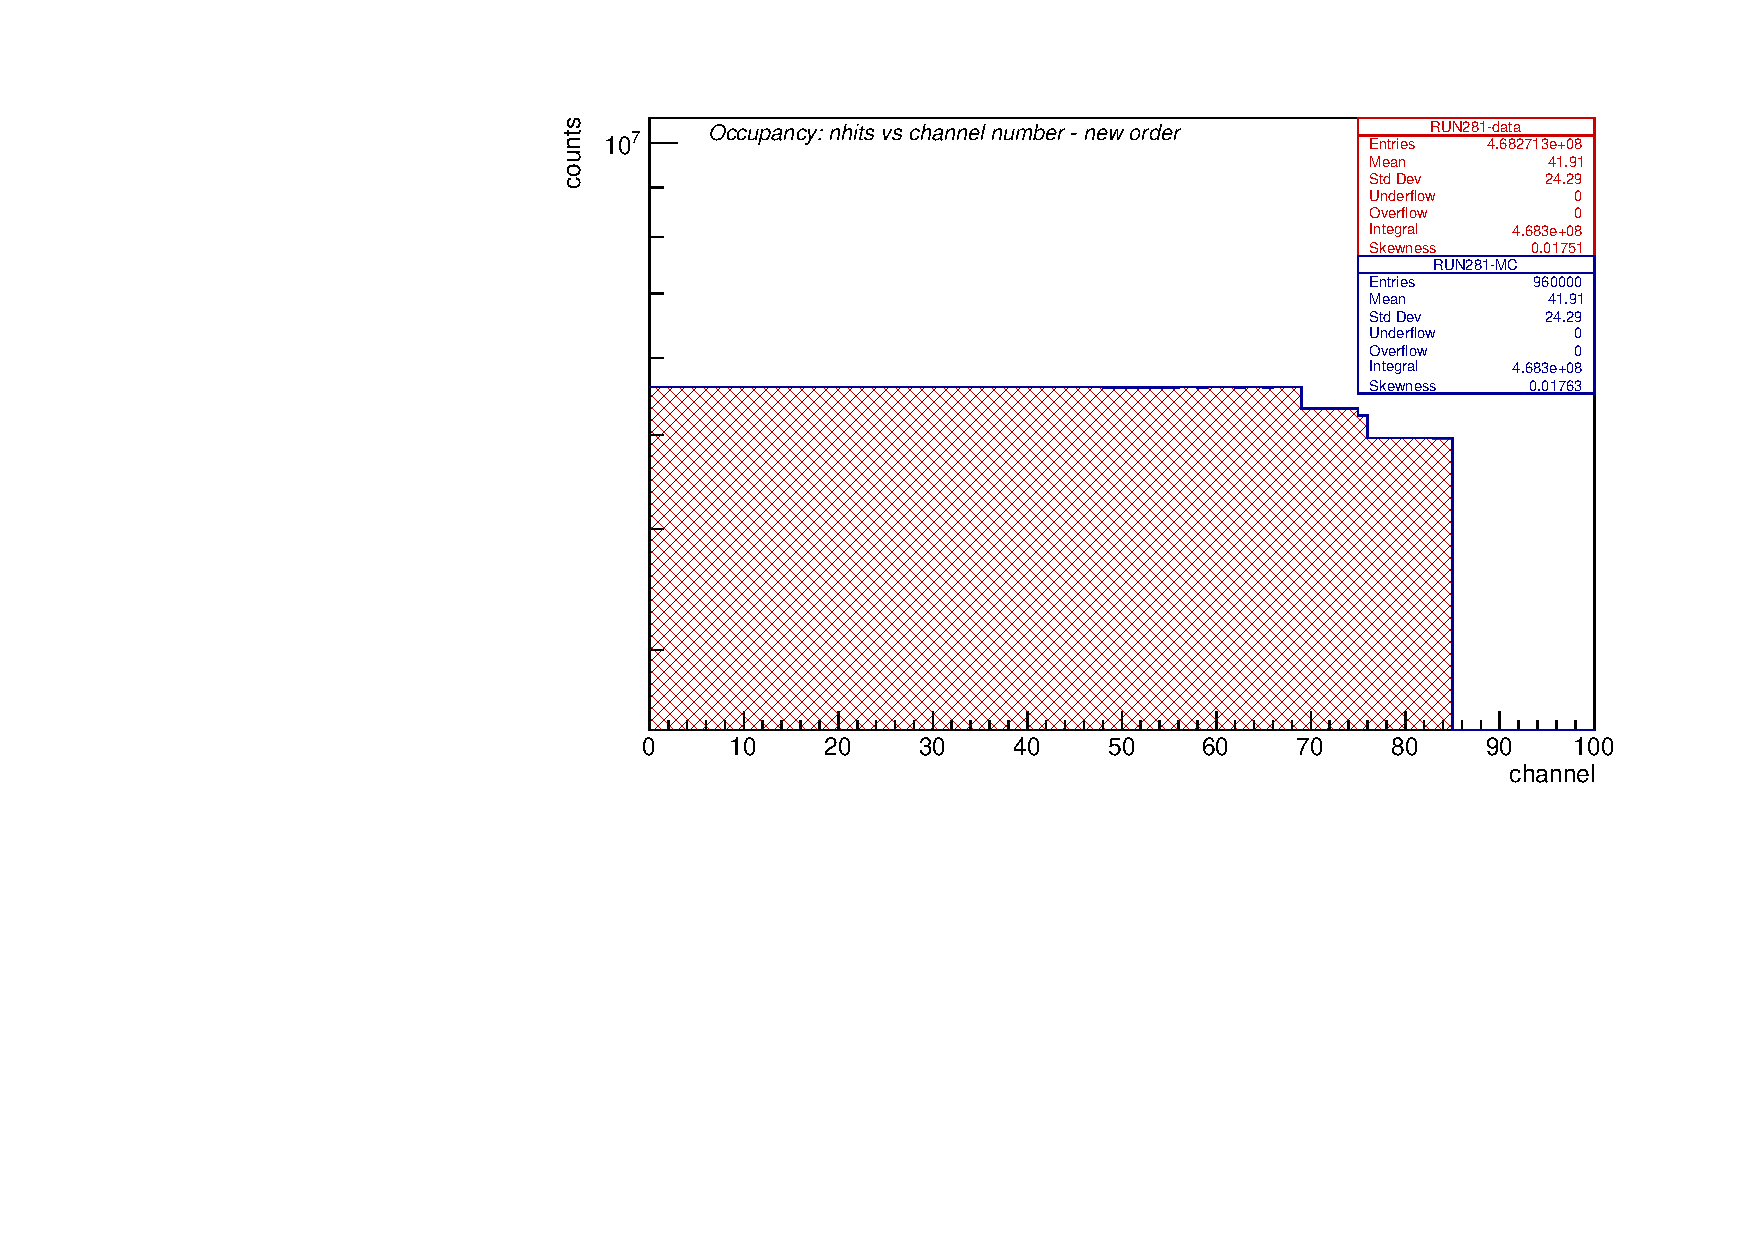
\includegraphics[width =0.8\textwidth]{figures/pdf/figure_00004_nhitsvschannel_roc_simulation_281}
\caption{Occupancy: number of hits versus channel. The ordering of channels adheres to the sequence prescribed by the Monte Carlo simulation.}
\label{fig:2}
\end{figure}
We can see a perfect adherence between data and simulation. We can interpret the histogram as it follows: the initial group of channels in the histogram,
corresponds to the ones in which we accumulate 4 hits (associated with the first FPGA) and 3 hits (associated with the second FPGA). 
Subsequently, we observe a contrasting group of channels where the pattern reverses, 3 hits from the first FPGA followed by 4 hits from the second FPGA.
We can observe a little jump in the middle and it is due to channel to channel time differences.
Time differences between channels are three order of magnitude less than the FPGA ones, so these little jumps are very few, in our case only one appears.
Lastly, the concluding cluster of channels is comprised of those collecting 3 hits from the first FPGA and 3 hits from the second FPGA.



\subsection{Number of hits}
\begin{figure}[!h]
\centering
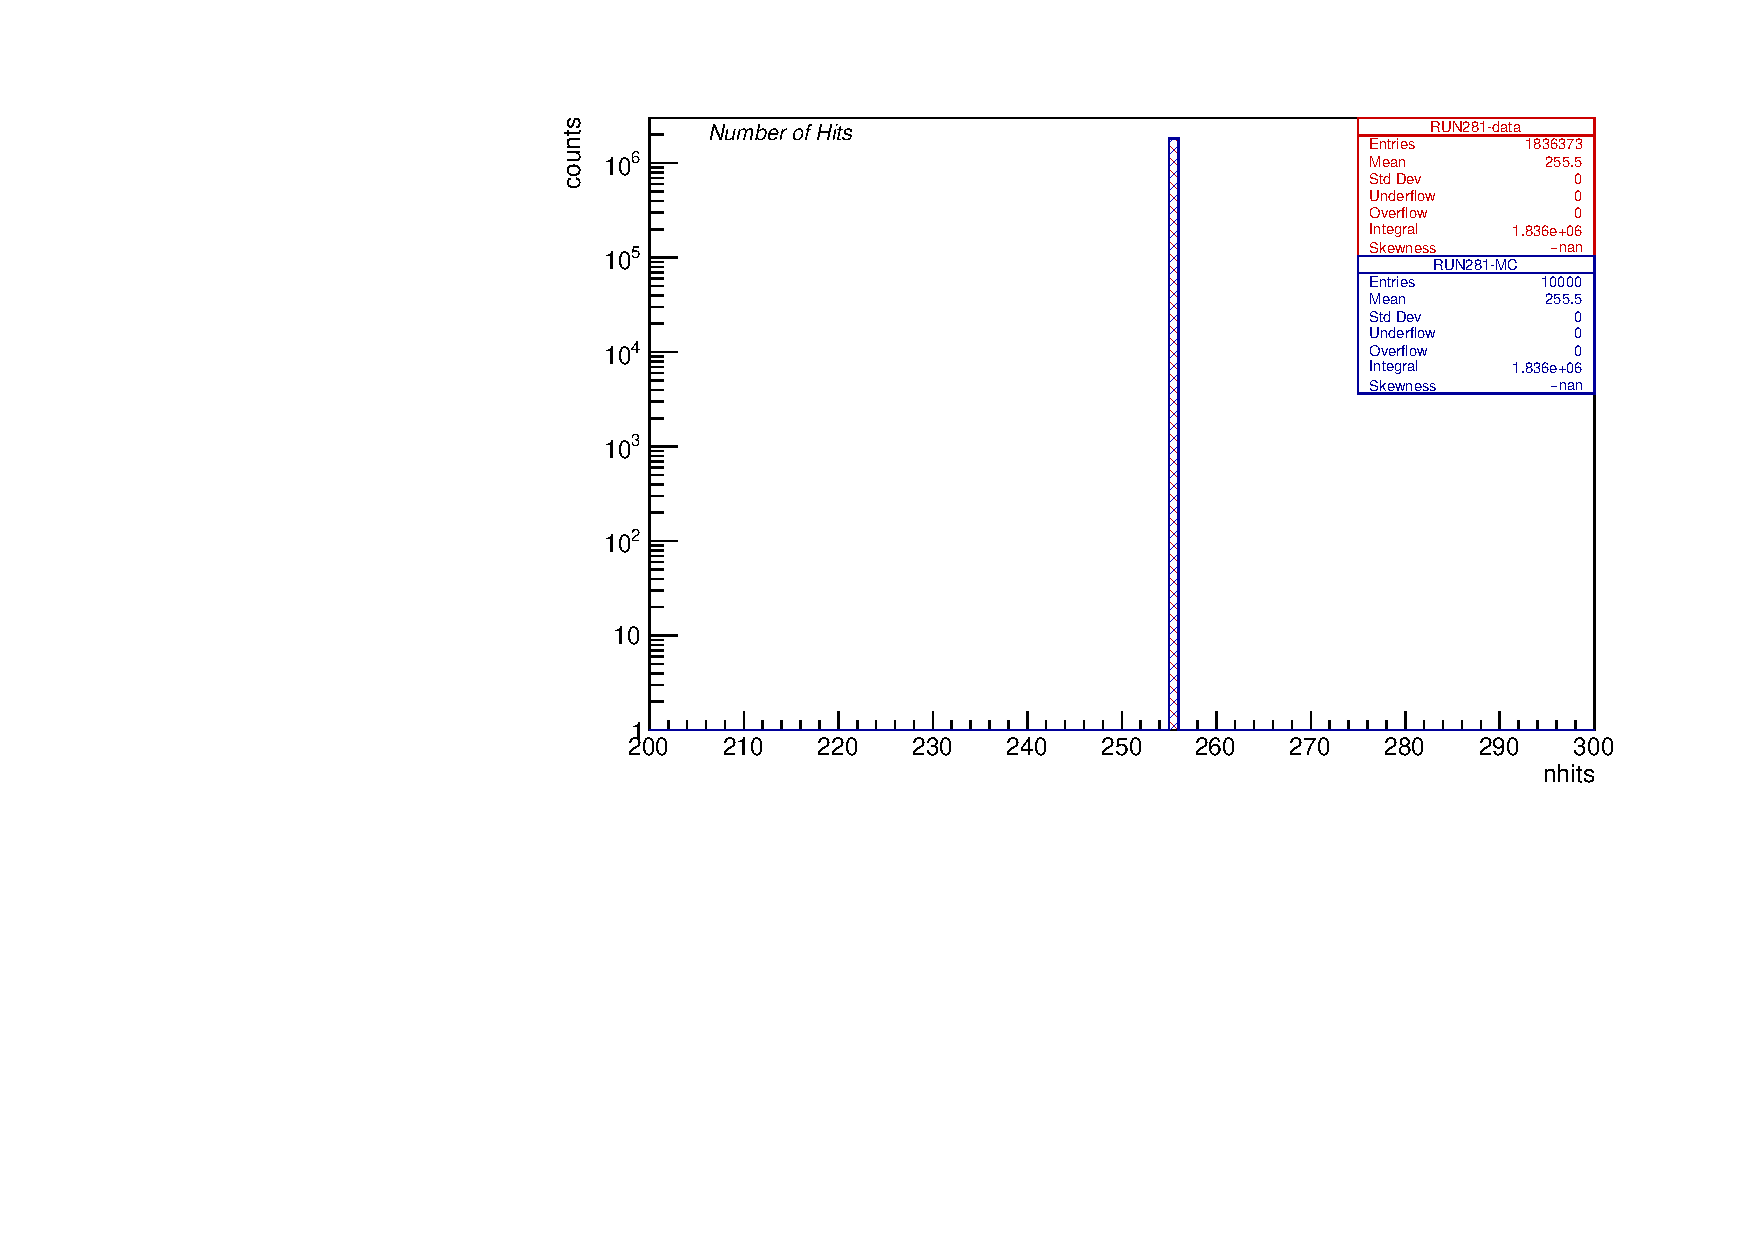
\includegraphics[width =0.8\textwidth]{figures/pdf/figure_00008_nhits_281}
\caption{Number of hits distribution.}
\label{fig:2}
\end{figure}


%%% Local Variables:
%%% mode: latex
%%% TeX-master: t
%%% End:
